\documentclass{report}
\usepackage[a4paper, total={6in, 8in}]{geometry}
\usepackage{amsmath}
\usepackage{bm}
\usepackage{pgfplots}
\usepackage{ amssymb }
\usepackage{color, soul}
\usepackage[backend=biber]{biblatex}
\addbibresource{references.bib}

%opening
\title{Literature Survey - (Title pending)}
\author{Ash}

\newcommand{\TODO}[1]{\sethlcolor{pink}\hl{(#1)}}
\newcommand{\FEEDBACK}[1]{\sethlcolor{green}\hl{Feedback: \\#1\\}}

\begin{document}
	
	\maketitle
	\thispagestyle{empty}
	\newpage
	\thispagestyle{empty}
	\tableofcontents
	\newpage
	\thispagestyle{empty}
	\listoffigures
	\newpage
	
	\chapter{Introduction}
	\textbf{Very brief background}
	Deep learning good for large data set.
	Motivation is to work with less training examples \\
	\textbf{Existing work on meta learning and continuous learning} \\
	\textbf{Gap the literature} \\
	\textbf{Describe the Problem}
	A system that can do continual learning. Refer to this doc:
	https://paper.dropbox.com/doc/Adding-classes-an-existing-classifier-RdKxXHh7M9OWbHvEvCCsV
	We want it to be scalable with respect to the number of classes
	So it should work faster than nearest neighbour based approaches for large number of classes \\
	\textbf{High level how you will solve it and why it is different from existing work} \\
	\textbf{Brief description of experimental setup} \\
	
	
	\chapter{Background}
	\TODO{Week 2} \\
	\FEEDBACK{1. The purpose of this chapter and how it connects to the previous and the next chapter \\
2. How does this chapter achieve its purpose, like the organization of the chapter, we first talk about this, then this,  etc.}
	Images are sources of highly-dimensional data for which humans have the incredible ability of understanding. Developing computer vision systems that perform to even a similar capacity to that of humans is an inherently difficult task. The gift of easily converting pixel values into meaningful concepts is a skill that computer vision experts have been attempting to transfer to computers for decades. \par
	The ability to quickly gain an understanding of a new concept is a uniquely human trait. Consider that after seeing a giraffe only once, most humans would be able to easily identify it in a humorous police line-up  -- perhaps after the theft of a monkey's balloon --  but the best image recognition systems over the years would be dependant on seeing many examples of giraffes. It is quite standard to present hundreds of examples of each new concept in order to learn which parts of the image data are unimportant noise, and which parts are characteristic. \par
	Modern techniques have made great advances in the application of meta-learning techniques (learning to learn) to few-shot learning; the task of having a computer vision system learn to recognize images from only a few labelled examples. While the results have been very encouraging, the problem of catastrophic forgetting persists. The challenge of continuous learning is to teach new classes to a system without interfering with the previously learnt tasks. \par
	
	\section{Hand Engineered and Learnt Features}
	\TODO{Week 2} \\
	Features are a general term for characteristic attributes which exist across all samples in a data-set or domain. These features were traditionally hand-engineered by machine learning experts, carefully selecting the base-components of which the data-set in question appears to comprise. \\
	A fundamental problem with hand-engineered features is that it imposes human knowledge onto a problem to be solved by a computer. Furthermore, key features for complex data such as images and video are incredibly difficult to ascertain -- especially if desiring generic, transferable features. With the rise of neural networks -- specifically CNNs, which will be discussed in detail later -- feature-learning has become the norm. This essentially takes the task of feature engineering and solves it in a data-driven manner.
	\FEEDBACK{Can you give some example pictures of what hand engineered features look like?}
	\section{Supervised Learning}
	\TODO{Week 2} 
	Supervised learning is a machine learning strategy whereby the target solution is presented after each training iteration. This differs from unsupervised learning in that unsupervised learning has no direct target to learn from and is used to find underlying commonalities or patterns in data. \\
	Supervised learning is the most commonly used method for image and video tasks, as typically the objective is to perform tasks where the target is well-defined. Common supervised learning tasks are \textit{image classification} - where the objective is to assign an input image a label from a fixed set of categories; \textit{localisation} - where the objective is to produce the coordinates of an object of interest from the input image; and \textit{detection} - which combines the previous two tasks. \\ \FEEDBACK{Maybe you can also mention regression.}
	There are a multitude of supervised and unsupervised learning problems, but as with almost all meta-learning strategies I will focus primarily on the supervised task of image classification using neural networks. \FEEDBACK{Maybe you can comment on the fact supervised learning is much more successful.}
	

	\section{Optimisation}
	\TODO{Week 2}
	\subsection{Loss} \label{loss:1}
	The process of optimising a machine learning system is to present it with a target of some sort -- either in the supervised or unsupervised setting -- and compute a numerical quantity called \textit{loss} or \textit{cost}. The loss is a scalar value which is representative of how ``badly'' the system has performed inference given the input image. It is the system's objective to minimise this value through some optimisation algorithm. The loss function is specifically chosen for the task at hand, \textit{cross-entropy} being a common choice for image classification tasks and \textit{mean-squared (L2) error}  for localisation. \\
	
	\subsubsection{Symbols}
	Before discussing loss functions, it's important to understand the inputs and outputs of a machine learning system when performing image classification. \\
	For a system that makes predictions between $N$ classes, its input is a vector of image features $\bm{x}$ - usually the raw pixel values. The system's output is a vector $\bm{\hat{y}}$ of length $N$, where each of the output values $\bm{\hat{y}}_i$ is a score for class $i$ being the correct answer. The loss $\mathcal{L}$, as described above, is a function of the predictions $\bm{\hat{y}}$ and the target values $\bm{y}$. \\
	The target values are typically encoded as a \textit{one-hot} vector of length $N$, which is all zeros with a 1 in the position of the correct class. \\
	
	\subsubsection{Softmax}
	As the system's outputs aren't normalised and thus cannot be interpreted as a true confidence measure, the outputs normally go through a softmax function $\sigma$.
	\begin{equation} \label{softmax:1}
	 \sigma(\bm{\hat{y}})_i = \frac{e^{\hat{y}_i}}{\sum_{k=1}^{N}e^{\hat{y}_i}} \\
	\end{equation}                                                              
	The softmax function (eq \ref{softmax:1}) squashes the arbitrary scores into a vector such that its values sum to $1$ and are each in the range $[0, 1]$. The resultant values can be interpreted as the probability of the input image falling into each of the classes. \\ \FEEDBACK{Can you give small table which has an example softmax distribution?}
	
	\subsubsection{Cross-Entropy Loss}	
	With the machine learning system producing a normalised probability distribution across classes, those values need be compared with the targets to produce a scalar loss value. 
	Cross-entropy loss, otherwise known as \textit{log loss}, penalises for differences between predicted values and targets, with the penalty growing harsher for further-away predictions as demonstrated in fig \ref{fig:cross-entropy:1}.\\
	For a vector of predictions $\bm{\hat{y}}$ and a one-hot target vector $\bm{y}$, the cross-entropy loss is:
	\begin{equation} \label{cross-entropy:1}
	 H(\bm{\hat{y}}, \bm{y}) = - \sum_{k=1}^{N}y_k log(\hat{y}_k) \\
	\end{equation}  
	For the special case of \textit{binary} cross-entropy (as shown in fig \ref{fig:cross-entropy:1}) where number of classes $N$ is 2, the network's outputs are generally reduced to a single scalar value and cross entropy calculated as:
	\begin{equation} \label{cross-entropy:2}
	 H(\hat{y}, y) = -(y log(\hat{y}) + (1 - y)log(1-\hat{y})
	\end{equation}
	\begin{figure}[!h]
		\centering
			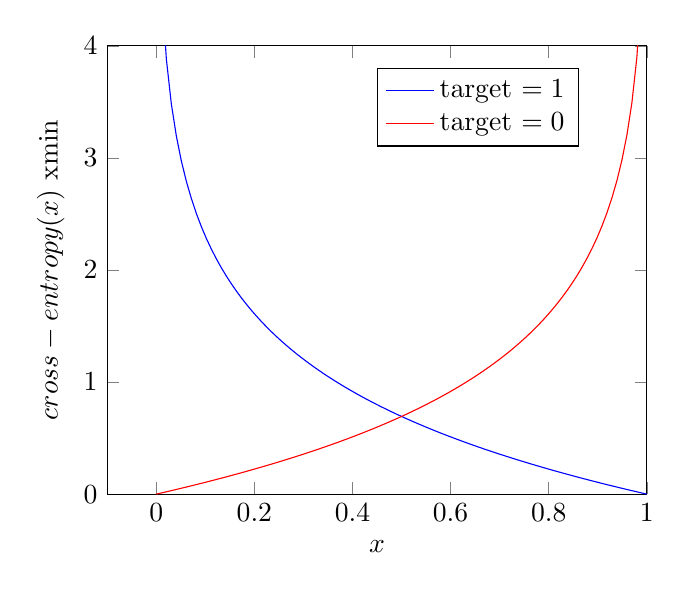
\begin{tikzpicture}
			\begin{axis}[ 
			xlabel=$x$,
			ylabel={$cross-entropy(x)$}
			xmin=0, xmax=1,
			ymin=0, ymax=4,
			legend style={at={(0.5,0.95)},anchor=north west}
			] 
			\addplot[domain=-0.01:1, color=blue, samples=100] 
				{-ln(x)};
			\addplot[domain=0:1, color=red, samples=100]
				{-ln(1 - x)};
			\addlegendentry{target $=1$}
			\addlegendentry{target $=0$}
			\end{axis}
			\end{tikzpicture}
			\caption{Binary Cross-Entropy}
			\label{fig:cross-entropy:1}
	\end{figure}
	
	\subsubsection{Mean-Squared Error (L2)}
	Mean-squared error is used for regression tasks, where the objective is to predict a quantitative value rather than a measure of probability. As L2 loss minimises the average error between the predictions $\bm{\hat{y}}$ and targets $\bm{y}$, the system learns to make predictions which lie in the mean position of these, which is generally ideal for regression tasks where there is one solution.\\
	\begin{equation} \label{mean-squared-error:1}
	 L2(\hat{\bm{y}}, \bm{y}) = \sum_{k=1}^{N}(y_k - \hat{y}_k)^2
	\end{equation}
	
	\section{Neural Networks}
	Artifical Neural Networks (\textit{ANNs}) are machine learning systems loosely inspired by the functioning of the biological neural networks of the brain. They are composed of artificial neurons which transmit signals from one another in the form of a non-linear function of the sum of the incoming inputs. ANNs model unknown functions of arbitrary complexity, with their representational power a function of their size. \par
	If we look at the structure of the simplest neuron possible $f_1$ (see fig \TODO{make figure}) we see that it is composed of two components - a weight $w_1$ and a bias $b_1$. Passing a value $x$ through a neuron $f_1$ is equivalent to computing the linear function $f_1(x) = w_1x + b_1$.
	If the outputs of this neuron are then passed into a similar neuron $f_2$, we end up with the composite function 
	\begin{align}
	 (f_2\circ f_1)(x) &= (w_2(w_1x + b_1) + b_2) \\
	 &= w_2w_1x + b_1w_2 + b_2	
	\end{align}
	which is still a linear function of $x$. This is true for any number of sequential neurons, meaning that any composition of linear neurons is only as good as a single neuron. Having the capacity to produce linear relationships is only useful if the function being modelled is, itself, a linear function. For more complex modelling tasks -- which are encountered more often than not -- non-linearities need to be introduced into the network. In making a neuron a non-linear function, the problem with composite functions noted above no-longer exists; adding additional neurons increases the representational power of the model. \par
	
	\subsection{Activation Functions / Non-Linearities}
	Activation functions (also known as non-linearities) are a critical component of neural networks as they add the capacity to model non-linear relationships. The inspiration for activation functions is drawn -- once again -- from the operation of biological neural networks, whereby neurons are only ``activated'' given sufficient input signal. In modern neural networks there are only a few activation functions regularly used: \par


	\begin{itemize}
		\item\textbf{Sigmoid} $= \frac{1}{1 + e^{-x}}$ : The Sigmoid activation function (also known as the \textit{logistic function}) has the nice property that $(\forall x \in \mathbb{R}) Sigmoid(x)\in(0, 1)$ which is useful as a way of normalising values, especially when the output is to be interpreted as a probability.
		
		\item\textbf{TanH} $= \frac{e^{2x} - 1}{e^{2x} + 1}$ : The hyperbolic tangent function is similar to sigmoid, but maps numbers to the range $(-1, 1)$.
		
		\item\textbf{ReLU} $= \begin{cases}
		0, & \text{if } x < 0 \\
		x, & \text{if } x \ge 0 \\
		\end{cases}$
		The Rectified Linear Unit maps numbers to the range $[0, \infty)$ and has the advantage that it is much more computationally efficient than the above two activation functions; in most cases it yields better results.
		\item\textbf{Leaky ReLU} $= \begin{cases}
		0.01x, & \text{if } x < 0 \\
		x, & \text{if } x \ge 0 \\
		\end{cases}$
		The Leaky Rectified Linear Unit operates like ReLU, but allows numbers less than zero to ``leak'' through - this is helpful during \textit{backpropogation}, which is discussed at length in section \ref{backprop:1}.
	\end{itemize}

	\subsection{Fully-Connected Layers}
	The arrangement and structure of neurons discussed thus far hasn't been very practical, in that we were only considering a chain of continuous neurons one after another with only one input and output. Neurons will typically receive multiple inputs and produce a weighted sum of those inputs. A neuron given $N$ inputs $x_i$ with weights $w_i$ and bias $b$ would then form the linear equation $w_1x_1 + w_2x_2 + ... + w_Nx_N + b$. \par
	For a system consisting of multiple inputs, we want to allow diverse interactions between them. This is achieved by what's known as a \textit{Fully-Connected Layer} of neurons, where each output from the previous layer is passed as input to each of the following layer's neurons. Networks are generally grouped into layers to provide a nice abstraction away from the hundreds or thousands of neurons inside, see fig \TODO{Create a nice picture of this}. \par \FEEDBACK{One of the useful purposes of this is that it allows you to customise to any output size easily.}

	\subsection{Stochastic Gradient Descent (SGD)} \label{sgd:1}
	\TODO{Week 2} \\
	An ANN begins with randomly generated weights and biases $\bm{W}$ and $\bm{B}$, which are collectively referred to as the ``parameters'' or ``weights'' and indicated by $\bm{\theta}$. The objective of an ANN is to select weights $\bm{\theta}$ that minimise the error computed by the loss function $\mathcal{L}$ (section \ref{loss:1}). Linear functions $f(\bm{x}, \bm{\theta})$ can be minimised by analytical techniques, but complex neural networks must be iteratively optimised by numerical methods. \\
	\TODO{Put in the argmax/minimisation objective function} \par
	With the loss between a prediction $\hat{y}$ and target $y$, we can compute the gradients of the parameters and make a small step in the direction which will reduce the loss for the given example (see fig \TODO{make loss surface figure}). When performing this operation over the entire data-set at once, this is known as gradient descent. This is usually not an option as the computational resources required for full gradient descent are prohibitive. If we instead repeat this operation for different examples until we have stabilised the loss to a low value, we have Stochastic Gradient Descent. The most common variant to this technique is known as Batch Gradient Descent, where instead of computing the loss and performing an update to the parameters on a per-example basis, the process is applied once per \textit{batch} of examples. It facilitates more stable learning, as the loss doesn't fluctuate as much as between single examples. Batch Gradient Descent is the basis for most ANN optimisation, although we'll discuss modern variants in section \ref{modern-dl:1}. \par

	\subsection{Gradients and Backpropagation} \label{backprop:1}
	\TODO{Week 2} \\
	We shall consider a general ANN $\sigma$ with $2$ fully-connected layers $f_1, f_2$ parameterised by $\bm{\theta} = \{\bm{\theta}_1, \bm{\theta}_2\}$ which can be represented as:
	\begin{align} \label{gradients:1}
	 \bm{\hat{y}} = \sigma(\bm{x}, \bm{\theta}) = f_2(f_1(\bm{x},  \bm{\theta}_1), \bm{\theta}_2)
	\end{align}
	That is, the input $\bm{x}$ is fed through layer $f_1$ then $f_2$. We will also consider an arbitrary loss function $\mathcal{L}$ which compares the predictions $\bm{\hat{y}}$ with targets $\bm{y}$ and produces a scalar loss value:
	\begin{align}
	 \mathcal{L}(\bm{\hat{y}}, \bm{y})
	\end{align}
	As the input $\bm{x}$ and target $\bm{y}$ is fixed, we may only change the parameters $\bm{\theta}$ to improve the loss. As explained in section \ref{sgd:1}, we wish to make incremental changes to our parameters where each change decreases our loss value. We do so by computing the gradient of the parameters with respect to the loss value:
	\begin{align}
	 \frac{\partial\mathcal{L}(\bm{\hat{y}},\bm{y})}
	 {\partial\bm{\theta}}
	\end{align}
	If we are to find the gradients of the loss function with respect to the final layer's weights, we will have the equation
	\begin{align}
	\frac{\partial\mathcal{L}(\bm{\hat{y}},\bm{y})}
	{\partial\bm{\theta}_2}
	\end{align}
	which is considered to be easily calculable. However, if we wish to find the gradient of weights further towards the start of the network, we cannot work those out directly and instead need to make use of the differentiation chain rule: \par
	\begin{align}
	\frac{\partial f}{\partial x} = \frac{\partial f}{\partial u} \frac{\partial u}{\partial x}
	\end{align}
	To find the gradient of the loss function with respect to the first layer's weights, and considering that $\frac{\partial\mathcal{L}(\bm{\hat{y}},\bm{y})}
	{\partial\bm{\theta}_2}$ is calculable, we simply need apply the chain rule as such:
	\begin{align}
	\frac{\partial\mathcal{L}(\bm{\hat{y}},\bm{y})}{\partial\bm{\theta}_1} =
	\frac{\partial\mathcal{L}(\bm{\hat{y}},\bm{y})}
	{\partial\bm{\theta}_2}
	\frac{\partial\bm{\theta}_2}
	{\partial\bm{\theta}_1} 
	\end{align}
	That is, once we know the gradient of the loss with respect to the second layer's weights, we can compute the gradient of the second layer's weights with respect to the first layer's weights and multiply the two to find the gradient of the loss with respect to the first layer's weights. This generalises to neural networks with any number of layers of differing types. This is an intuitive relationship, as we are essentially calculating the compound contribution that a change in any one parameter's value will have on the final output -- the loss.  \par
	This technique used since the 1970s \parencite{backprop} is aptly named \textit{backpropagation of error gradient}, as it involves the propagation of the gradient of the error -- or loss -- from the end of the network back. \par
	Returning to the concept of SGD (section \ref{sgd:1}) which was introduced on a conceptual level, we can now delve deeper into the application of the algorithm. Assuming that we have computed the gradient of each parameter in the network for the given examples in our batch, we can visualise this as a ``loss landscape'', whereby moving the parameters down-hill results in a reduction in the loss. Adjusting a parameter by the negative of the gradient will result in a ``step'' that moves the parameter closer to a local minimum, with the objective to reach the lowest point possible. A configurable hyperparameter is the \textit{learning-rate}, commonly represented by $\alpha$, which is the ``size'' of the step to take - that is, the coefficient of the negative of the gradient to apply (eqn. \ref{sgd:1}). \par
	\begin{align} \label{sgd:1}
		\bm{\theta} = \bm{\theta} - \alpha \Delta_{\bm{\theta}} \mathcal{L}(\bm{\theta}, \bm{\hat{y}}, \bm{y})
	\end{align}
	\textit{For brevity we will from now write the gradient of the parameters $\bm{\theta}$ with respect to the loss function $\mathcal{L}$ as $\Delta_{\bm{\theta}} \mathcal{L}(\bm{\theta})$.} \\
	The problem that is quickly encountered is how large a value to set the learning rate $\alpha$. Too small a step and it will take a long time to reach the minimum; too large and you may over-shoot it  (see fig \TODO{make a figure}). The example in  (fig \TODO{make a figure}) is a very low-dimensional loss landscape where the corect direction to move seems very logical, but higher dimensional spaces with a greater number of parameters result in complex landscapes with many local minima. We also want to slow down when nearing the bottom of a minimum so we can properly reach the lowest point. If we take this into consideration, and the fact that for any mini-batch the loss landscape will be different due to noise in small sample sizes, choosing a fixed learning rate becomes problematic. In practice, many people simply set up a learning rate schedule, where they decrease the learning rate at intervals, but it is hard to get right. It is with this in mind that adaptive optimizers came about. \\
	
	
	\subsection{Adaptive Optimizers}
	If we consider a data-set whereby each mini-batch has some noise but that there is an optimal parameterisation for the entire set, we could visualise the loss landscape as shifting slightly for each mini-batch, but where there is a common direction towards which most samples will lead. Standard SGD will just apply a fixed step-size for all updates which leads the parameters to oscillate along the greatest descent angle, regardless of past updates. \par
	
	\subsubsection{SGD with Momentum}
	It is with the idea of a consistent optimization direction that momentum comes into play. This is a technique of updating parameters while taking past updates into consideration to find the ``common direction'' in which to move. This is done by using an update vector which intuitively acts like the momentum of a ball rolling down a hill. For any update step, the direction vector is updated with a scaled contribution from the current gradient direction, and that vector is used to update the parameters. It essentially dampens oscillating movement, as the direction vector compounds contributions in the same direction as given in the following equation
	\begin{align}
		\bm{v}_t &= \gamma \bm{v}_{t-1} + \alpha \Delta_{\bm{\theta}} \mathcal{L}(\bm{\theta}) \\
		\bm{\theta}_t &= \bm{\theta}_{t-1} - \bm{v}_t
	\end{align}
	where $\gamma$ is the momentum term which indicates how much movement we wish to carry forward from previous time-steps.
	
	\subsubsection{Nesterov Accelerated Gradient Descent}
	If we consider momentum to compound the previous slopes such as a ball rolling down a hill, we end up with a problem where the momentum may cause the parameters to overshoot the minimum. Nesterov Accelerated Gradient Descent pre-emptively considers post-step parameters and makes adjustments to the step \textit{actually} taken. It does so by approximating the position after a momentum parameter update ($\bm{\theta} - \gamma\bm{v}_{t-1}$), and computes the loss gradient not with respect to the current parameters, but to the approximate future position of the parameters. This optimisation strategy essentially glances into the future and makes a pre-emptive correction.
	\begin{align}
		\bm{v}_t &= \gamma \bm{v}_{t-1} + \alpha \Delta_{\bm{\theta}} \mathcal{L}(\bm{\theta} - \gamma\bm{v}_{t-1}) \\
		\bm{\theta}_t &= \bm{\theta}_{t-1} - \bm{v}_t
	\end{align}
	
	\subsubsection{Adagrad}
	Adagrad is the first of the true ``adaptive'' optimizers, in that it adjusts the learning rate on a per-parameter basis, taking past gradients into consideration. The Adagrad update rule is
	\begin{align} \label{adagrad:1}
		\theta_{t, i} &= \theta_{t-1, i} - \frac{\gamma}{\sqrt{g_{t, i} + \epsilon}} \mathcal{L}(\theta_{t, i})
	\end{align}
	where $\theta_i$ is the $i$th parameter, $\gamma$ is the learning rate, $g_i$ is the square of the sum of the squares of the gradients with respect to $\theta_i$ up to step, $\epsilon$ is a small number to avoid dividing by zero, and $\mathcal{L}(\theta_i)$ is the gradient of the loss with respect to $\theta_i$. This optimizer has the benefit that while rarely performing as well as SGD with well-chosen hyperparameters, the Adagrad's default learning rate of $0.01$ consistently yields very good results.
	
	\subsubsection{Adadelta and RMSprop}
	The accumulation of squared gradients in the denominator of Adagrad means that that the learning rate continues shrinking and eventually becomes small enough to entirely stop training. Adadelta seeks to resolve this by instead of storing the accumulated sum of squared gradients, keeping a running average 
	\begin{align}
		E[g^2]_{t, i} = \gamma E[g^2]_{t-1, i} + (1 - \gamma)g^2_{t, i}
	\end{align}
	and updating equation \ref{adagrad:1} to be
	\begin{align}
		\theta_{t, i} &= \theta_{t-1, i} - \frac{\gamma}{\sqrt{E[g^2]_{t, i} + \epsilon}} \mathcal{L}(\theta_{t, i})
	\end{align}
	RMSprop \parencite{rmsprop} is in effect identical to Adadelta, and were both developed to address the diminishing learning rate proplem of Adagrad.
	
	\subsubsection{Adam}
	Adaptive Moment Estimation (Adam) \parencite{adam} builds from the previous adaptive optimizers by not only storing exponentially decaying averages of past squared gradients $v_{t,i}$, but by also keeping an exponentially decaying average of past gradients $m_{t,i}$ -- note the lack of the word ``squared''. 
	\begin{align}
		m_{t, i} &= \beta_1 m_{t-1, i} + (1 - \beta_1)g_{t, i} \\
		v_{t, i} &= \beta_2 v_{t-1, i} + (1 - \beta_2)g^2_{t, i}
	\end{align}
	where $\beta_1$, $\beta_2$ are hyperparameters the proportion of past information carried forward, with the default values typically working well in practice. Replacing $E[\bm{g}^2]$ with $\bm{v}$, $\mathcal{L}(\bm{\theta})$ with $\bm{m}$, and a small change to the square-root we end up with
	\begin{align}
		\theta_{t, i} = \theta_{t-1, i} - \frac{\gamma}{\sqrt{v_{t, i}} + \epsilon} m_{t, i}
	\end{align}	
	While not the most recent (I have omitted a few other adaptive optimizers), Adam is rapidly becoming the most frequently used optimizer for its consistent convergence and ease-of-use.
	
	\section{Dealing with Small Training Data Sets}
	\subsection{Overfitting}
	\subsection{Transfer Learning}
	\subsection{Few-Shot Learning}
	\subsection{Meta Learning}
	\textit{Break into meta training, testing, episodes, etc.}
	\section{Continuous Learning}
	\textit{Catastrophic forgetting}
	\section{Modern Deep Learning Architectures} \label{modern-dl:1}
	\subsection{Convolutional Neural Networks}
	\subsection{Recurrent Neural Networks}
	
	\chapter{Related Works}
	\section{Meta Learning}
	Approaches in meta learning with neural networks are generally groupd into three categories.
	\subsection{Model Based}
	\subsection{Metric Based}
	\subsection{Optimization Based}
	\section{Continuous Learning}
	\chapter{Proposal}

	\printbibliography
	
	


\end{document}
